\documentclass[../Report.tex]{subfiles}
\usepackage[italian]{babel}
\graphicspath{ {../../Images/} }

\begin{document}
    \chapter{Studio di fattibilità}
    \section{Contesto di utilizzo}
    Questa sezione mira ad identificare gli utenti della piattaforma e i loro compiti, in particolare enfatizzando la relazione tra i loro obiettivi (user goal) e le mansioni svolte (task). Inoltre, vengono individuati vincoli ambientali e tecnici rilevanti per le successive fasi di design.
        
        \subsection{Utenti previsti}
        Ci aspettiamo che gli utenti destinatari, che andranno ad utilizzare il sito Gioco.it, sono bambini che vogliono giocare ai vari mini giochi contenuti in esso, sorvegliati però dai loro genitori/tutori che si preoccupano per la loro sicurezza. Quindi, in questo caso il responsabile (i genitori/tutori) è diverso dall'utente (bambino).\\
        Abbiamo individuato due segmenti target di riferimento, in sintesi:
        \begin{itemize}
            \item Bambini di età compresa fra i 3 e i 18 anni che abbiano un minimo di dimestichezza con il dispositivo e con la navigazione internet. Interessati a giocare ai vari mini giochi presenti sul sito.
            \item Uomini/donne, il cui reddito è medio-basso (tutti ormai abbiamo almeno un dispositivo con navigazione internet) e che abbiano una buona dimestichezza con il dispositivo e con la navigazione internet. Interessati a far giocare il bambino a giochi prevalentemente educativi e bloccando quelli che ritengono inopportuni per l'età del bambino.
        \end{itemize} 

        \subsection{Compiti previsti}
        Durante le interviste sono emerse una serie di “idee per compiti” ricorrenti. Elaboriamo queste idee per produrre un elenco dei compiti più plausibili che il nostro sistema supporterà:
        \begin{itemize}
            \item Creazione di un profilo
            \item Login e logout dal sistema (anche con google o facebook)
            \item Visualizzare i giochi in tendenza
            \item Visualizzare i giochi in base a varie categorie e sottocategorie
            \item Giocare ai vari mini giochi
            \item Ricercare i giochi per nome e categoria
            \item Utilizzo di un parental control (filtro età, tempo di gioco e categorie)
            \item Commentare i giochi
            \item Aggiungere i giochi ai preferiti
            \item Aggiungere amici, rimuovere amici 
            \item Creare una conversazione
            \item Commentare la conversazione di un amico
            \item Modificare il proprio avatar 
        \end{itemize}

        \subsection{Vincoli ambientali e tecnici}
        \begin{itemize}
            \item \textbf{Vincoli tecnici:} trattandosi di una piattaforma web, è necessario che l'utente disponga di una connessione internet. Quindi supponiamo che tutti i nostri utenti possiedano almeno un personal computer (desktop o laptop) o smartphone con una connessione ad internet.
            \item \textbf{Vincoli ambientali:} la piattaforma è pensata per essere utilizzata nel tempo libero, pertanto l'ambiente di utilizzo più comune sarà la propria abitazione o un ambiente altrettanto confortevole e accogliente, senza alcun vincolo di tempo.
        \end{itemize}
        Ci aspettiamo quindi, che la maggior parte degli utenti utilizzi il sistema a proprio piacimento, in modo rilassato, esplorativo e possibilmente senza obiettivi.

    \section{Personas}
    \label{section: personas}
    Partendo dai nostri target segments, presentiamo quattro personas plausibili, due per ciascun target segments. Partiamo con il protagonista (Mirko) e poi forniamo altri tre personaggi secondari (Claudio, Gaetano e Simona).\\

    \begin{table}[H]
        \begin{tabular}{|c|l|p{7cm}|}
            \hline
            \multirow{5}{*}{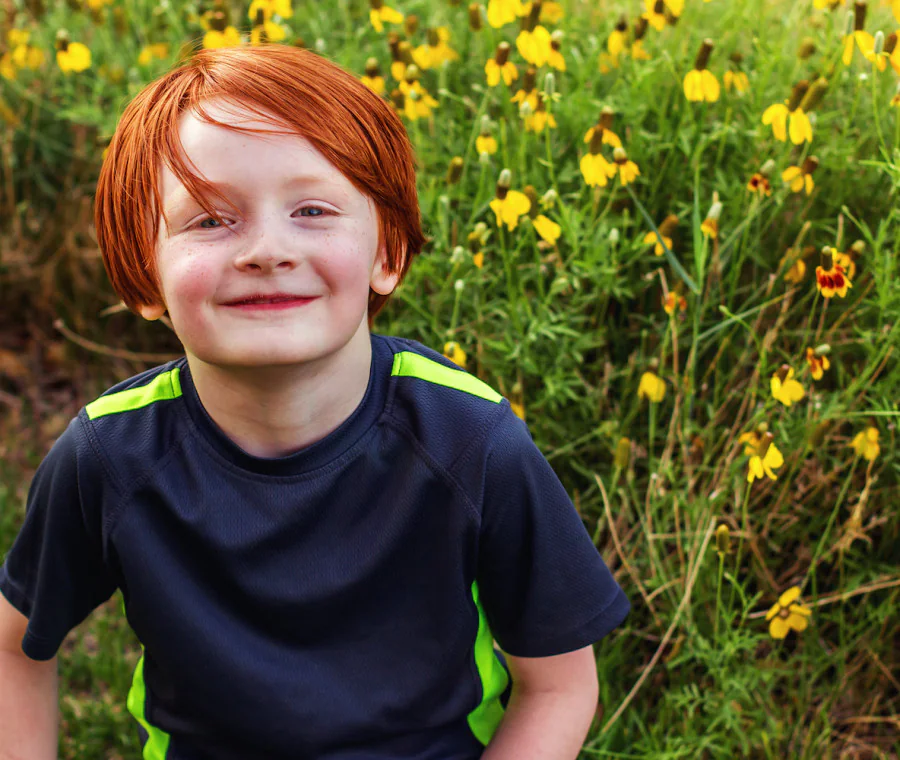
\includegraphics[width=5cm, height=5cm]{Gaetano.jpg}} 
                & \textbf{Nome:} & Gaetano Artico\\ \cmidrule{2-3}
            & \textbf{Età:} & 8 \\ \cmidrule{2-3}
            & \textbf{Stato civile:} & Nubile \\ \cmidrule{2-3}
            & \textbf{Occupazione:} & \makecell{Studente \\ Mantenimento da parte dei genitori} \\ \cmidrule{2-3}
            & \textbf{Abilità tecinche:} &  Sa usare il computer grazie agli insegnamenti di suo padre ed è un maestro nel riconoscere dinosauri.\\
            \hline
        \end{tabular}
    \end{table}

    \subsubsection{Descrizione}
    Gaetano è un bambino di 8 anni, frequenta la terza elementare, ed è l'unico figlio di mamma Daniela, barista, e papà Fabio, dentista. È un bambino molto perspicace ed attento, ama la natura e gli animali e infatti per il suo quinto compleanno il padre gli ha regalato un bellissimo Golden Retriver di nome Pippo. La sua più grande passione sono i dinosauri, infatti riesce a riconoscerne tantissimi grazie all'innumerevole quantità di libri e video che studia a riguardo.
    Gaetano va due volte a settimana a seguire corsi di piscina, spinto dalla passione della madre, ex nuotatrice amatoriale.\\
    Suo padre preferirebbe che imparasse giocando, ed è proprio per questo che gli permette di utilizzare il suo computer fisso per giocare a giochi educativi.

    \vspace{1.5cm}

    \begin{table}[H]
        \begin{tabular}{|c|l|p{7cm}|}
            \hline
            \multirow{5}{*}{
\includegraphics[width=5cm, height=5cm]{Claudio.jpg}} 
                & \textbf{Nome:} & Claudio Esposito\\ \cmidrule{2-3}
            & \textbf{Età:} & 45 \\ \cmidrule{2-3}
            & \textbf{Stato civile:} & Sposato \\ \cmidrule{2-3}
            & \textbf{Occupazione:} & \makecell{Medico di base \\ 70.000€ reddito netto annuo} \\ \cmidrule{2-3}
            & \textbf{Abilità tecinche:} &  Conosciuto in tutta la città per la sua professionalità e competenza. Ha un MacBook Pro che utilizza per lavorare e un computer fisso a casa per vedere film e seguire corsi di aggiornamento.\\
            \hline
        \end{tabular}
    \end{table}

    \subsubsection{Descrizione}
    Claudio è un medico di 45 anni, sposato con una bellissima parrucchiera di nome Jennifer e hanno un bimbo di 6 anni, Salvatore, molto intelligente e che ama il calcio. È uno dei più bravi medici di base della sua città e lo conoscono tutti con il soprannome di "Claudjello", per le sue origini partenopee. Oltre al suo lavoro, gli piace cimentarsi nell'informatica e utilizza il suo computer fisso per seguire corsi di aggiornamento e guardare film e serie tv. Una delle sue serie tv preferite è l'anime Naruto, infatti lui e Salvatore passano ore davanti al pc a guardarne le puntate.\\
    Claudio ci tiene molto all'educazione del figlio, ed è per questo che vorrebbe far giocare suo figlio a dei giochi principalmente educativi.

    \vspace{1.5cm}

    \begin{table}[H]
        \begin{tabular}{|c|l|p{7cm}|}
            \hline
            \multirow{5}{*}{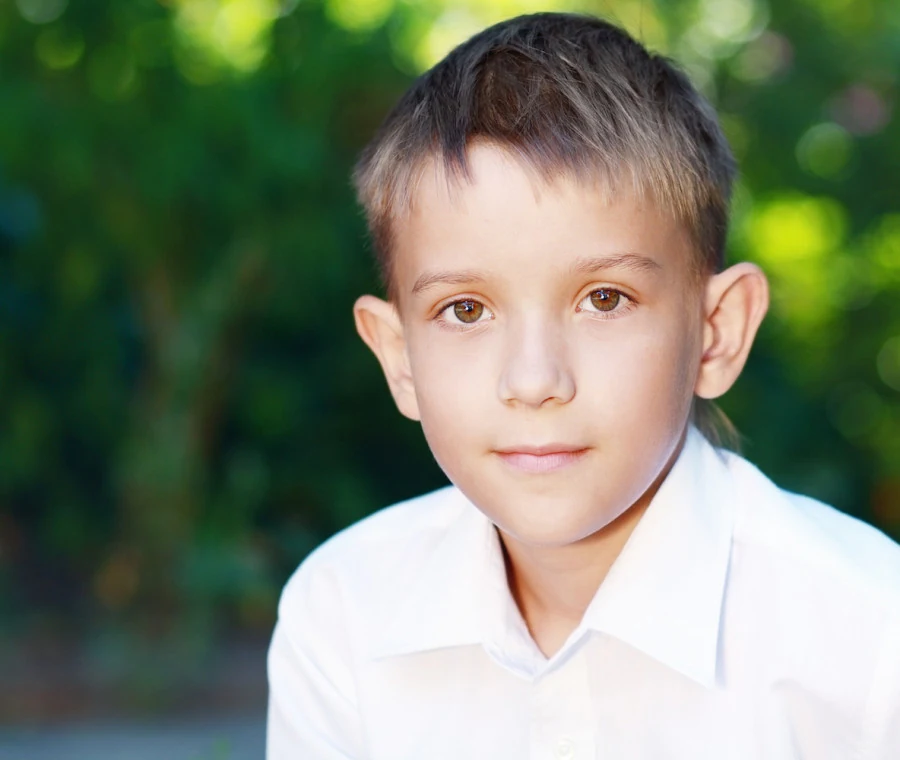
\includegraphics[width=5cm, height=5cm]{Mirko.jpg}} 
                & \textbf{Nome:} & Mirko Rossi\\ \cmidrule{2-3}
            & \textbf{Età:} & 12 \\ \cmidrule{2-3}
            & \textbf{Stato civile:} & Nubile \\ \cmidrule{2-3}
            & \textbf{Occupazione:} & \makecell{Studente \\ Mantenimento da parte dei genitori} \\ \cmidrule{2-3}
            & \textbf{Abilità tecinche:} & Usa il laptop della madre per fare ricerche scolastiche o per giocare. Gioca spesso con gli amici ed è imbattibile nei giochi d'azione, principalmente gli sparatutto. \\
            \hline
        \end{tabular}
    \end{table}

    \subsubsection{Descrizione}
    Mirko è un ragazzino di 11 anni che frequenta la quinta elementare nella scuola del suo paese. Mirko è un grande appassionato di calcio, gioca nelle sezioni giovanili della squadra della sua città il Manfredonia, è un attaccante ed il suo idolo è l'attaccante del Milan Ibrahimovic.  Ha una sorella di 15 anni che è appassionata di moda. La madre, Susanna, lavora come commercialista in uno studio del loro piccolo borgo cittadino. Il padre, Antonio, esercita la professione di elettricista e spesso è fuori casa. Dopo aver fatto i compiti, Mirko, utilizza il laptop della madre per giocare a diversi videogiochi. La madre, essendo molto apprensiva nei confronti del figlio, tiene molto alla sua educazione, pertanto vorrebbe una maggiore sicurezza sugli usi del suo laptot.

    \vspace{1.5cm}

    \begin{table}[H]
        \begin{tabular}{|c|l|p{7cm}|}
            \hline
            \multirow{5}{*}{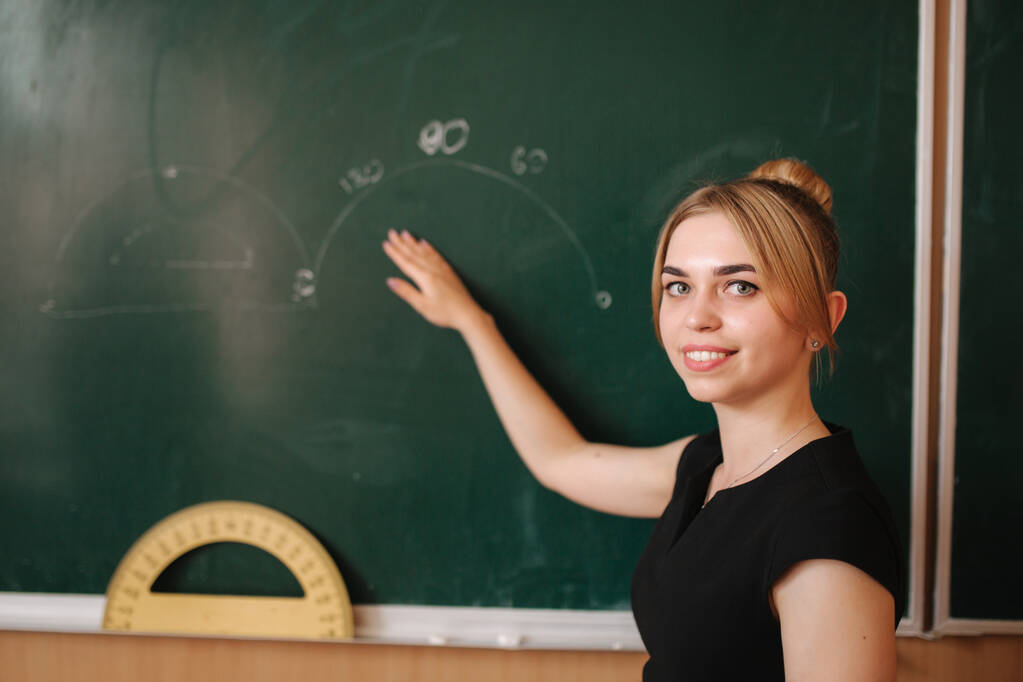
\includegraphics[width=5cm, height=5cm]{Simona.jpg}} 
                & \textbf{Nome:} & Simona Guerra\\ \cmidrule{2-3}
            & \textbf{Età:} & 30 \\ \cmidrule{2-3}
            & \textbf{Stato civile:} & Nubile \\ \cmidrule{2-3}
            & \textbf{Occupazione:} & \makecell{Insegnante di scuola primaria \\ 17.000€ reddito netto annuo} \\ \cmidrule{2-3}
            & \textbf{Abilità tecinche:} &  Ama innovare il modo di insegnare. Abile con il pennello, utilizza il suo laptop per comprare quadri all'asta e per seguire nuovi corsi sui metodi di insegnamento.\\
            \hline
        \end{tabular}
    \end{table}

    \subsubsection{Descrizione}
    Simona è un'insegnate della scuola primaria di 30 anni. È l'unica figlia di una cassiera in pensione di 68 anni e di un operaio di 62 anni, con i quali vive tuttora. Si è diplomata al liceo classico ed in seguito si è laureata in Scienze della formazione all'Università di Bologna.\\
    Ama stare con i bambini, infatti ora insegna nella scuola primaria del suo paese. I suoi hobby principali sono la pittura e leggere romanzi, anche se passa svariate ore su Instagram. Vorrebbe proporre al preside della sua scuola di poter far giocare i suoi alunni ad alcuni giochi educativi su internet, ma la sua paura è che potrebbero finire a giocare anche a giochi non adatti alla loro età.

    \section{Scenari}
    Procediamo ora a fornire uno scenario di utilizzo plausibile per ciascuno dei nostri personaggi, nella speranza di comprendere meglio la relazione tra obiettivi personali e compiti coinvolti.

    \subsection{Basta sparare (Mirko)}
    In questi giorni la scuola di Mirko è chiusa per le vacanze di Natale, quindi ha più tempo libero per dedicarsi ai suoi videogiochi preferiti sul sito Gioco.it, tra cui Subway Clash 2. Questo gioco, per l'età di Mirko, è abbastanza cruento e poco educativo, in effetti venne a conoscenza del sito e del gioco tramite suo cugino Daniele di 16 anni. Susanna, la madre di Mirko, venendo poi a conoscenza delle attività ricreative di Mirko online (Gioco.it), ha capito di intervenire cercando di bloccare l'accesso a questi giochi violenti. Decise così di accedere al sito, creare un profilo a Mirko (con i propri dati) e tramite l'utilizzo del parental control, in modo intuitivo, è riuscita a filtrare solo i giochi per ragazzi dai 10 anni in giù.

    \subsection{Enigma Matematico (Simona)}
    Simona ha sentito parlare di Gioco.it da un suo amico che lo  ha già usato una o due volte, per curiosità e noia. Ha appena giocato a "A caccia di parole", un gioco educativo dove l'obiettivo è trovare tutte le parole nascoste all'interno di un puzzle.\\
    Un giorno ha deciso di proporre al preside della scuola dove insegna, di poter far giocare i suoi alunni con dei giochi educativi nel laboratorio d'informatica e lui ha accettato subito. Il primo giorno in cui Simona accompagna i suoi alunni al laboratorio, dopo che essi cominciarono a giocare, si rese conto che alcuni alunni giocavano a diversi giochi violenti. Lei prese subito in mano la situazione, fece accedere ad ogni alunno con il suo profilo personale e, data la grafica molto semplice ed intuitiva, riuscì a settare il filtro per giochi di categoria "matematica". Alla fine dell'ora i ragazzi si divertirono molto e impararono anche a fare le addizioni.

    \subsection{Addio ricerca di storia (Gaetano)}
    Gaetano è capitato sul sito Gioco.it navigando su internet per un banner pubblicitario durante una ricerca scolastica, infatti ha lasciato perdere la ricerca e ha passato tutto il pomeriggio a giocare con i vari mini giochi sul sito.\\
    Il giorno dopo è tornato a casa con una nota della maestra per non aver svolto la ricerca di storia. Il padre, Fabio, si è infuriato e ha deciso di controllare le attività di suo figlio al computer di casa. Ha così deciso di aprire il sito Gioco.it, è riuscito i modo semplice a creare un profilo per Gaetano ed inserire i limiti di età per i diversi giochi e anche un limite di tempo per usufruire di essi. Ora Gaetano ha capito che non deve passare troppo tempo davanti ai videogiochi e soprattutto che sono molto più costruttivi i giochi educativi.

    \subsection{Un'esultanza che mi rappresenta (Mirko)}
    Nella ricreazione a scuola Mirko parlava con il suo compagno di banco Alessandro a riguardo della partita del Milan della sera prima. A tal proposito Alessandro gli dice che suo padre gli ha fatto vedere una bellissima foto di Ibrahimovic che esulta per il goal segnato, Mirko pensa subito che vuole averla! Dopo averla ricevuta dal padre di Alessandro decide subito di volerla impostare come foto profilo per il suo account di Gioco.it. Apre quindi il suo profilo e tramite pochi semplici ed intuitivi click riesce ad impostarla. I suoi amici di giochi tifosi dell'Inter saranno neri di rabbia!

    \subsection{Amici di giochi (Claudio)}
    Claudio, tornando a casa dal lavoro, ha sentito parlare di Gioco.it dal padre di un amico del figlio, Marco, dicendogli che è stato proprio Salvatore a fargli conoscere il sito e che oramai Marco passa le giornate a giocare agli sparattutto. Claudio, tornando a casa, controlla la cronologia del computer fisso di casa e vede che negli ultimi giorni Salvatore ha passato troppo tempo a giocare ai videogiochi, principalmente agli sparattutto. Allora Claudio decide di creare un profilo a Salvatore ed applicare i modo semplice e veloce delle restrizioni per non farlo giocare a troppi giochi violenti. Decide anche di invitare, tramite il sito, il suo amico Marco in modo da potersi confrontare con classifiche e commenti sui vari videogiochi e anche per fare tenere sotto controllo Marco da suo padre.


    \subsection{Intense discussioni (Mirko)}
    Mirko sta giocando ad un gioco chiamato "Subway Surf" su Gioco.it, un gioco Arcade in cui è spaventosamente bravo. A seguito però di un consiglio del suo migliore amico Alessandro decide di fare un tentativo e di giocare ad un gioco molto simile, chiamato "Temple Run". Mirko si scopre un asso anche in questo gioco, proprio poichè i due sono veramente molto simili, continua però a preferire "Subway Surf" per la grafica molto più bella. Si chiede allora quale sia il parere dei suoi amici in merito e decide quindi di aprire una discussione sul suo profilo e scrive:\\
    "Subway Surf vs Temple Run, amici quale vi piace di piu?". Scoprirà infine che quasi tutti i suoi amici, come lui preferiscono "Subway Surf".


\end{document}